% Figure: Crossover ratio vs array size
\begin{figure}[H]
\centering
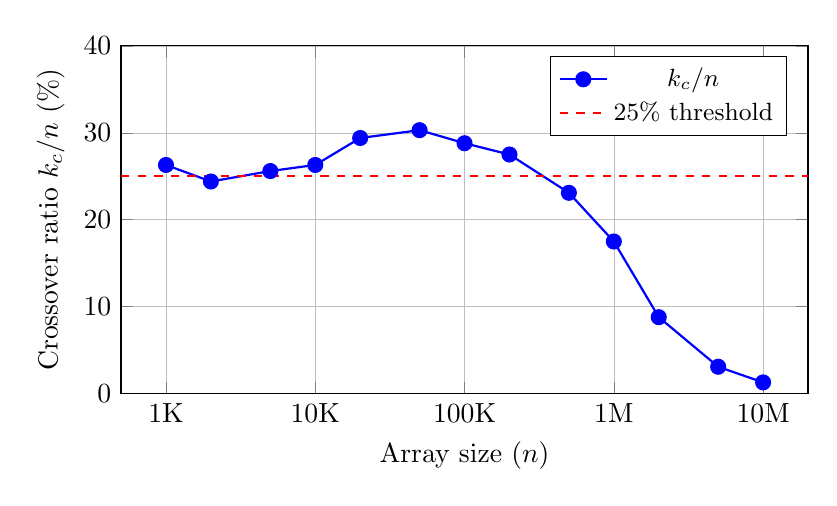
\begin{tikzpicture}
\begin{axis}[
    width=0.85\textwidth,
    height=6cm,
    xlabel={Array size ($n$)},
    ylabel={Crossover ratio $k_c / n$ (\%)},
    xmode=log,
    log basis x=10,
    xmin=500, xmax=20000000,
    ymin=0, ymax=40,
    ytick={0, 10, 20, 30, 40},
    yticklabels={0, 10, 20, 30, 40},
    xtick={1000, 10000, 100000, 1000000, 10000000},
    xticklabels={1K, 10K, 100K, 1M, 10M},
    legend pos=north east,
    legend style={font=\small},
    grid=both,
    grid style={line width=0.1pt, draw=gray!30},
    major grid style={line width=0.2pt, draw=gray!50},
]

% Crossover ratio line
\addplot[color=blue, mark=*, thick, mark size=2.5pt] coordinates {
    (1000, 26.3) (2000, 24.4) (5000, 25.6) (10000, 26.3) 
    (20000, 29.4) (50000, 30.3) (100000, 28.8) (200000, 27.5) 
    (500000, 23.1) (1000000, 17.5) (2000000, 8.8) (5000000, 3.1) (10000000, 1.3)
};

% Reference line at 25%
\addplot[color=red, dashed, thick] coordinates {
    (500, 25) (20000000, 25)
};

\legend{$k_c / n$, 25\% threshold}
\end{axis}
\end{tikzpicture}
\caption{Crossover ratio $k_c / n$ as a function of array size. DeltaSort outperforms 
Native sort when the dirty fraction is below this curve. The 25\% rule of thumb 
(dashed line) is conservative for small-to-medium arrays but optimistic for very 
large arrays where the crossover drops significantly.}
\label{fig:crossover-ratio}
\end{figure}
